\chapter{XGBoost}
\label{ch-xgboost}

This paper is based on the original
XGBoost paper Ref.\cite{xgboost-2016}
and the excellent StatQuest videos 
(highly recommended) \cite{statquest-xgb}.

Extreme Gradient Boosting (XGBoost) (Chen, Guestrin, 2016)
improves
gradient boosting (Friedman, 1999)
in a number of ways, such as by using a quadratic 
rather than linear approximation
for the variational function.

In XGBoost, one 
calculates a sequence 
of functions
where each function tries to 
correct the errors of the previous function. Then 
a series (i.e., linear combination) of 
those functions yields an estimate $\haty^\s$
of the target attribute $y^\s$.
As will
be shown in this chapter, XGBoost can be used 
in two cases: Regression
(continuous target attribute)
and Binary Classification
(binary target attribute)\footnote{
XGBoost can also be used for
classification into more than two classes, as
long as a suitable Divergence function
 can be defined.}.
An implementation of the XGBoost algorithm
is available as open source. It's
written in C++, with Python
and R interfaces.

Boosting (see this chapter on XGBoost
and
Chapter \ref{ch-adaboost} on AdaBoost)
and bagging
(see Chapter \ref{ch-rforest} on Random Forest)
are two methods
of building a classifier function
from an ensemble
of classifier functions.
These two methods are most commonly
applied to dtrees: Boosting for an ensemble of
small dtrees, and Bagging for a random
forest (which
is an ensemble
of dtrees that are usually much more
complicated than small dtrees).

\section{Divergences}
To set up
a cost function
for XGBoost,
we begin by defining
2 types of ``divergences"
and
calculating the first and second derivatives
of those divergences:

\begin{itemize}
\item
{\bf Divergence for regression}
(i.e., continuous classification,
continuous target attribute). For $x,y\in \RR$
\beq
D_{reg}(x,y)=\frac{1}{2}(x-y)^2
\eeq

\item
{\bf Divergence for binary classification} (i.e., binary
target attribute). 
For $p,q\in[0,1]$.
\beqa
D_{bc}(p,q) &=&-\{
p\ln q +(1-p)\ln(1-q)\}
\\
&=&CE(\{p, 1-p\}\parallel\{q, 1-q\})
\eeqa
The cross-entropy $CE()$
is defined in Chapter \ref{ch0-conventions}.
\end{itemize}

\begin{claim}
\beq
\partial_\haty D_{reg}(y, \haty)=
\haty-y
\eeq

\beq
\partial^2_\haty D_{reg}(y, \haty)=1
\eeq

\beq
D(y, \haty+ h)
\approx D(y, \haty)
+ (\haty-y) h
+\frac{1}{2} h^2
\eeq
\end{claim}
\proof
Obvious.
\qed

Recall from Section \ref{sec0-smoid}
in Chapter \ref{ch0-conventions}
that

\beq
\haty =\smoid(\lodds(\haty))
\eeq

Let us abbreviate  $s()=\smoid()$
and $l()=\lodds()$ so

\beq
\haty=s(l(\haty))
\;.
\eeq



\begin{claim}\footnote{Note that $D_{bc}(y,\haty)\neq D_{bc}(\haty, y)$; i.e.,
$D_{bc}$ is not symmetric in its two
arguments. Normally $0<\haty <1$ and $y\in \bool$.
Since the log is applied 
only to the second argument, 
to avoid logs
of zero,
it is better to have $\haty$ as
the second argument.} 

\beq
\partial_l D(y, \haty(l))=\haty-y
\eeq

\beq
\partial^2_l D(y, \haty(l))= \haty(1-\haty)
\eeq

\beq
D(y, \haty(l+\Delta l))
\approx D(y, \haty(l))
+ (\haty-y)\Delta l
+\frac{1}{2}\haty(1-\haty)(\Delta l)^2
\eeq
\end{claim}
\proof

\beqa
\pder{ D(y,s)}{s}
&=&
-\partial_s\{
y\ln s + (1-y)\ln (1-s)\}
\\
&=&
-\;\frac{y}{s} + \frac{1-y}{1-s}
\\
&=&
\frac{-y(1-s)+(1-y)s}{s(1-s)}
\\
&=&
\frac{-y+s}{s(1-s)}
\eeqa

Recall that 
$\smoid'(l)=\smoid(l)[1-\smoid(l)]$ so
\beq
\pder{s}{l}=s(1-s)
\;.
\eeq

\beq
\pder{ D(y,s)}{l}=
\pder{s}{l}\;\;
\pder{ D(y,s)}{s}
=
-y+s=
-y +\haty
\eeq

\beq
\frac{\partial^2 D(y,s)}
{\partial l^2}
=\pder{s}{l}=s(1-s)
\eeq
\qed



\section{Minimizing Cost function
for single tree}
Let

$\s\in \Sigma$ be an individual in a population $\Sigma$

$x^\s\in S_\rvx$ be a feature vector 
$x^\s=(x^\s_i)_{i=0,1, \ldots, nf-1}$


$t\in\{0,1, \ldots, nt-1\}$ be the tree index

$\call_t$ be the set of leafs of
tree $t$

$\ell\in \call_t$ be a leaf in tree $t$

$w_t^{\ell}\in \RR$

$f_t:S_\rvx\rarrow \RR$

$\ell_t:\Sigma\rarrow \call_t$, $\ell_t(\Sigma)=\call_t$.

$\ell_t(\s)$ be the leaf of individual $\s$ in tree $t$

$
\Sigma_t^\ell=
\{
\s\in\Sigma : \ell_t(\s)=\ell\}
$

Define the function $f_t$ by
\beq
f_t(x^\s)= \sum_{\ell\in\call_t}
w_t^\ell\indi(\s\in \Sigma_t^\ell)
=
w_t^{\ell_t(\s)}
\;.
\eeq
$f_t(x^\s)$ gives 
the output
value for tree $t$
and feature vector $x^\s$.

Define the {\bf cost function}
for tree $t$ as follows

\beq
\calc_t
=\sum_\s D(\haty^\s_t
,y^\s)
+
\underbrace{\sum_{\ell\in \call_t}
\left[
\gamma +\frac{\lam}{2}(w_t^\ell)^2
\right]
}_{\text{regulator}}
\;,
\label{eq-xgb-cost-fun}
\eeq
where $\gamma>0, \lam>0$ are  regulator
parameters.



The estimate $\haty^\s_t$, using
trees from 0 to $t$,
of the target attribute $y^\s$, is
defined by

\beqa
\haty^\s_0&=& f_0(x^\s)=\text{arbitrary constant, 
XGBoost default for this is 0.5}
\\
\haty^\s_1&=&f_0(x^\s)+f_1(x^\s)
\\
\haty^\s_2&=&f_0(x^\s)+f_1(x^\s)+f_2(x^\s)
\\
\vdots
\\
\haty^\s_t&=&
\sum_{t'\leq t}f_{t'}(x^\s)
=
\haty^\s_{t-1} + f_t(x^\s)
\eeqa

In the cost function $\calc_t$,
we approximate the divergence $D()$
by a second order Taylor approximation:
\beqa
D(y^\s,\haty^\s_t)
&=&
D(y^\s,\haty^\s_{t-1}+
\underbrace{f_t(x^\s)}_\delta)
\\
&\approx&
D(y^\s,\haty^\s_{t-1})
+ a^\s_t \delta
+ \frac{1}{2}b^\s_t \delta^2
\\
&=&
D(y^\s,\haty^\s_{t-1})
+
a^\s_t w_t^{\ell_t(\s)}
+ \frac{1}{2}b^\s_t (w_t^{\ell_t(\s)})^2
\;,
\eeqa
where

\beq
a^\s_t=
[\partial_{\haty}D(y^\s,\haty)]_{\haty=\haty^\s_{t-1}}
\;,
\eeq

\beq
b^\s_t=
[\partial^2_{\haty}D(y^\s,\haty)]_{\haty=\haty^\s_{t-1}}
\;.
\eeq
$a^\s_t$ is called $g$ for gradient
and $b^\s_t$ is called $h$ for Hessian
in Ref.\cite{xgboost-2016}.
Table \ref{tab-xgb-derivatives}gives the values 
for $a^\s_t$ and
$b^\s_t$ for
Regression (reg) and Binary classification (bc).



Define the {\bf residual}
for tree $t$ and individual $\s$ by
\beq
r^\s_t=y^\s-\haty^\s_{t-1}
\;.
\eeq

% Please add the following required packages to your document preamble:
% \usepackage[table,xcdraw]{xcolor}
% If you use beamer only pass "xcolor=table" option, i.e., \documentclass[xcolor=table]{beamer}
\begin{table}[h!]
\centering
\begin{tabular}{|
>{\columncolor[HTML]{ECF4FF}}l |l|l|}
\hline
 & \cellcolor[HTML]{ECF4FF}\begin{tabular}[c]{@{}l@{}}Regression \\
 ($y^\s\in\RR ,\haty^\s_t \in\RR$, $D=D_{reg}$)\end{tabular} & \cellcolor[HTML]{ECF4FF}
\begin{tabular}[c]{@{}l@{}}Binary Classification \\ ($y^\s\in \bool$, $\haty^\s_t
\in [0,1]$, $D=D_{bc}$)\end{tabular} \\ \hline
$a^\s_t$ & $\haty^\s_{t-1}-y^\s=\text{neg.residual}$ & $\haty^\s_{t-1}-y^\s=\text{neg.residual}$ \\ \hline
$b^\s_t$ & 1 & $\haty^\s_{t-1}(1-\haty^\s_{t-1})$ \\ \hline
\end{tabular}
\caption{The first ($a^\s_t$) 
and second ($b^\s_t$) derivatives for
Regression (reg) and Binary classification (bc).}
\label{tab-xgb-derivatives}
\end{table}

Note that
\beq
\sum_\s= \sum_{\ell\in\call_t}\sum_{\s\in \Sigma_t^\ell}
\;.
\eeq
Define

\beq
A_t^\ell=\sum_{\s\in \Sigma_t^\ell} a^\s_t
\eeq
and

\beq
B_t^\ell=\sum_{\s\in \Sigma_t^\ell} b^\s_t
\;.
\eeq


Now we can rewrite the cost function as
\beqa
\calc_t
&=&
\underbrace{\sum_\s D(\haty^\s_{t-1}, y^\s)}_{\calk}
+
\sum_{\ell\in \call_t}
\left[
A_t^\ell w_t^\ell + \frac{1}{2}B_t^\ell (w_t^\ell)^2
\right]
+
\sum_{\ell\in \call_t}
\left[
\gamma +\frac{\lam}{2}(w_t^\ell)^2
\right]
\\
&=&
\sum_{\ell\in \call_t}
\left[\gamma+
A_t^\ell w_t^\ell +
\frac{1}{2}(B_t^\ell+\lam) (w_t^\ell)^2
\right]
\;\;\;\text{(absorbed $\calk$ into $\gamma$)}
\eeqa

The cost function $\calc_t$
can be minimized over $w^\ell_t$:

\beq
0=
\delta \calc_t
=
\sum_{\ell\in \call_t}
\delta w_t^\ell
\left[
A_t^\ell + (B_t^\ell + \lam)w_t^\ell
\right]
\eeq
Therefore,
the cost is minimized when

\beq
w_t^\ell= \frac{-A_t^\ell}{B_t^\ell + \lam}
\;.
\eeq
The optimum cost is

\beq
\calc_t=
\sum_{\ell\in \call_t}
\underbrace{
\left[
\gamma-
\underbrace{
\frac{(A^\ell_t)^2}
{2(B_t^\ell + \lam)}
}_{SS_t^\ell}
\right]
}_{\calc^\ell_t}
\eeq




$SS_t^\ell$ is called the {\bf similarity score} for
leaf $\ell$ and tree $t$.
Note that an increase in similarity
 decreases  the cost.

\section{Leaf Splitting}
Suppose
leaf $\ell_0$ splits into leafs $\ell_L$
and $\ell_R$. Then

\beq
\Sigma_t^{\ell_0}=\Sigma_t^{\ell_L}\cup\Sigma_t^{\ell_R},
\;\;\;
\Sigma_t^{\ell_L}\cap\Sigma_t^{\ell_R}=\emptyset
\;
\eeq
so

\beq
A_t^{\ell_0}=A_t^{\ell_L} + A_t^{\ell_R}
\eeq
and

\beq
B_t^{\ell_0}=B_t^{\ell_L} + B_t^{\ell_R}
\;.
\eeq
Hence,

\beq
\calc_t^{\ell_j}=
\gamma-
\frac{(A_t^{\ell_j})^2}{2(B_t^{\ell_j} + \lam)}
\;\;\;\text{for $j=L,R$}
\eeq

\beq
\calc_t^{\ell_0}=
\gamma-
\frac{(A_t^{\ell_L}+A_t^{\ell_R})^2}
{2( B_t^{\ell_L}+ B_t^{\ell_R} +\lam)}
\eeq

Define the {\bf XGBoost branch Gain} for a binary tree
branch by
\beqa
GainXGB
&=&
\calc_t^{\ell_0}-
\calc_t^{\ell_L} -\calc_t^{\ell_R}
\\
&=&
\underbrace{
\left\{
SS_t^{\ell_L}
+SS_t^{\ell_R}
-SS_t^{\ell_0}\right\}
}_{\Delta SS_t}
-\gamma
\eeqa



\begin{figure}[h!]
\centering
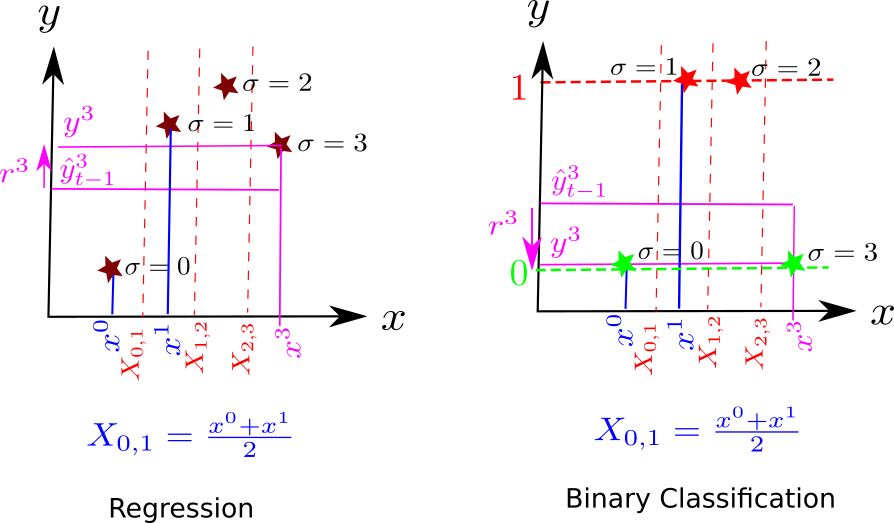
\includegraphics[width=6in]
{xgboost/xgb-partitions.png}
\caption{Plot of
target attribute $y^\s$ 
versus a feature
vector $x^\s$
with a single component.
More generally, 
the feature vector 
 $x^\s=(x^\s_j)_
{j=0,1, \ldots, nf-1}$
can have multiple components
called features or attributes.
The left plot
refers to a population 
of 4 individuals and regression
so $y^\s, \haty^\s\in \RR$.
The right plot 
refers to a population 
of 4 individuals and binary classification
so $y^\s\in\bool, \haty^\s\in [0,1]$.
$X_{j,j+1}$ for $j=0,1,2$ is
the average between 2 
adjacent values of $x^\s$.
 } 
\label{fig-xgb-partitions}
\end{figure}

\begin{figure}[h!]
\centering
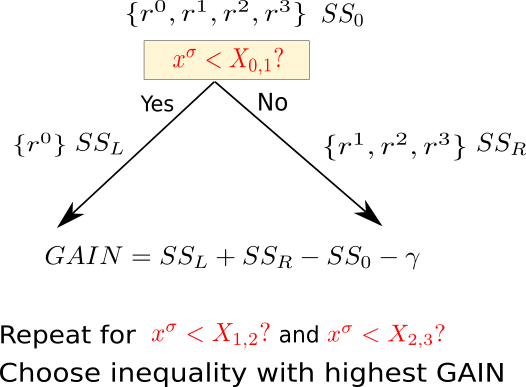
\includegraphics[width=3in]
{xgboost/xgb-splitting.png}
\caption{This 
figure refers to the situation of 
 Fig.\ref{fig-xgb-partitions}.
Out of all
allowed tree branches, we 
choose the one with the highest gain.
 } 
\label{fig-xgb-splitting}
\end{figure}

By splitting a leaf,
we create a new binary branch
with 2 new leafs.
We successively add new 
branches to the tree until
some stopping criterion is satisfied.
We continue adding branches to the tree
as long as they have a positive gain,
and 
as long as the number of levels is smaller
than an upper bound input parameter (XGBoost's default 
maximum number of tree levels is six).
XGBoost also rules out leafs
that have a denominator quantity
 $B^\ell_t$ (called the {\bf cover})
smaller than a lower bound  input parameter.
This branching 
process
is illustrated
in Figs.\ref{fig-xgb-partitions}
and \ref{fig-xgb-splitting}.


\section{Pruning}
If we raise $\gamma$
or raise $\lam$,  branches
that previously had positive gain
may acquire a negative gain.
Get rid 
of branches
from highest level that now have negative gain.
This will generate new branches.
Get rid of new branches
from the highest level that have
negative gain. Continue
this process until all
highest level branches have 
positive gain.
This may reduce a tree
to a single node
or even rule out the entire
tree.

$\lam$ measures {\bf level of insensitivity}
to observations, and $\gamma$ measures
{\bf level of tree simplicity}.



\section{Feature Binning}

For really large population sizes $|\Sigma|$, 
it is convenient to bin the 
set $\{x^\s_i:\s\in \Sigma\}$
for each $i$. 

A common
bin type is quantiles. 
Quantiles are bins $[X_{j-1}, X_j]$
 for $j=0, 1, 
\ldots, nbins-1$ that 
all contain approximately
the same number of points.
For example, 
in Fig.\ref{fig-xgb-splitting},
with 1 point quantile bins,
use $[X_{j-1}, X_j]$ for $j=0,1,2,3$.
With 2 point quantile bins,
use $[X_{j-1}, X_j]$ for $j=0,1$.

Use the right edge 
of each bin as the $X_j$ in the question 
 $x^\s<X_j?$,
and choose the question which
yields the highest gain.


 


\section{Final estimate of
target attribute}

In this section,
we will
give a formula for the 
final estimate
of the target attribute.
Previously, we set
the learning rate $\eta$ to one.
Here we restore $\eta$
to an arbitrary value 
between 0 and 1.

Instead of using 

\beq
f(x^\s)=\sum_{t=0}^{nt-1} f_t(x^\s)
\;,
\label{eq-xgb-approx-wo-eta}
\eeq
we will use 

\beq
f(x^\s)=\sum_{t=0}^{nt-1} 
 (\eta)^t f_t(x^\s)
\;,
\label{eq-xgb-approx-eta}
\eeq
where $\eta\in [0,1]$ is called 
the {\bf learning rate}.
This has the effect
of compensating for the $f_t$'s
with $t>nt-1$ that would
 have been included
had we used an infinite series.
Also, think of Eq.(\ref{eq-xgb-approx-wo-eta})
as
an approximation  (a truncated Taylor
expansion in powers
of $\Delta x$) of a function $f(x+\Delta x)$,
and think of Eq.(\ref{eq-xgb-approx-eta})
as an analogous approximation of the function 
$f(x+\eta \Delta x)$.

For the case of Regression, we get:

\beqa
f(x^\s)
&=&
\sum_t (\eta)^t\left(
\frac{- A_t^{\ell_t(\s)}}
{B_t^{\ell_t(\s)} + \lam}
\right)
\;.
\eeqa

For the case of Binary Classification,
 we get

\beq
f(x^\s)=\sum_{t=0}^{nt-1}(\eta)^t
\underbrace{
\smoid\underbrace{\left(
\frac{- A_t^{\ell_t(\s)}}
{B_t^{\ell_t(\s)} + \lam}\right)
}_{\text{lodds(probability)}}
}_{\text{probability}}
\;.
\eeq

\section{Bnet for XGBoost}




\begin{figure}[h!]
$$
\xymatrix{
\vec{y}\ar@/_1pc/[rr]\ar@/_1pc/[rrr]
&\ul{\ell}_0 \ar@/_2pc/[dd]\ar@/_2.5pc/[ddd]\ar@/_3pc/[dddd]
&\ul{\ell}_1 \ar@/_2pc/[dd]\ar@/_2.5pc/[ddd]\ar@/_3pc/[dddd]
&\ul{\ell}_2 \ar@/_2pc/[dd]\ar@/_2.5pc/[ddd]\ar@/_3pc/[dddd]
\\
\vec{x}\ar[r]\ar@/_1pc/[rr]\ar@/_1pc/[rrr]
&[\ul{\haty}^\s_0]_{\s\in\Sigma}\ar[rdd]
\ar[rd]\ar[ru]
&
[\ul{\haty}^\s_1]_{\s\in\Sigma}\ar[rdd]
\ar[rd]\ar[ru]
&
[\ul{\haty}^\s_2]_{\s\in\Sigma}
\\
\ul{\vecy}\ar[r]\ar@/_1pc/[rr]\ar@/_1pc/[rrr]
&[\ul{A}^\ell_0]_{\ell\in\call_0}
&
[\ul{A}^\ell_1]_{\ell\in\call_1}\ar@/_2.5pc/[dd]
&
[\ul{A}^\ell_2]_{\ell\in\call_2}\ar@/_2.5pc/[dd]
\\
&[\ul{B}^\ell_0]_{\ell\in\call_0}
&
[\ul{B}^\ell_1]_{\ell\in\call_1}\ar[d]
&
[\ul{B}^\ell_2]_{\ell\in\call_2}\ar[d]
\\
\vec{x}\ar@/_1pc/[drrrr]
\ar@/_1pc/[rr]\ar@/_1pc/[rrr]
&f_0\ar[drrr]\ar@/_2pc/[uuu]
&f_1\ar[drr]\ar@/_2pc/[uuu]
&f_2\ar[dr]\ar@/_2pc/[uuu]
\\
&&&&f
}$$
\caption{Bnet for XGBoost assuming $nt=3$. 
Nodes that appear
multiple
times (namely $\ul{\vecx}$ and $\ul{\vecy}$ )
should be considered the same node,
drawn multiple times for  clarity.
The parameters $\lam, \gamma, \eta$ are 
taken to be global. Recall that
$\ell_t:\Sigma\rarrow \call_t$.
From the function $\ell_t()$, we can derive
its range $\call_t=\{\ell_t(\s):\s\in\Sigma\}$),
and 
$\Sigma^\ell_t=\{\s\in\Sigma: \ell_t(\s)=\ell\}
$ for all $\ell\in \call_t$.}
\label{fig-xgb-bnet}
\end{figure}

Fig.\ref{fig-xgb-bnet}
gives our bnet for the XGBoost algo
assuming $nt=3$.
The TPMs, printed in blue,
for this bnet, are as follows:


For $t=0$, 
$\ell_0$ describes a single node 
``tree" such that $\ell_0(x^\s)=f_0(x^\s)=0.5$
for all $\s\in\Sigma$.
For $t\geq 1$, 
\beq\color{blue}
P(\ell_t|\vec{y},
[\haty^\s_{t-1}]_\s)=
\begin{array}{l}
\text{build tree $\ell_t$ using 
$y^\s$ and $\haty^\s_{t-1}$
for all $\s\in \Sigma$.}
\\
\text{$\lam$ and $\gamma$ are used here.}
\end{array}
\eeq

\beq\color{blue}
P([\haty^\s_t]_\s\cond f_t , \vec{x})=
\prod_{\s\in\Sigma}
\indi(\;\;\;\haty^\s_t= f_t(x^\s)\;\;\;)
\eeq

\beq\color{blue}
P([A^\ell_t]_{\ell\in\call_t}\cond
\vec{y}, [\haty_{t-1}^\s]_\s,\ell_t
)=
\prod_{\ell\in\call_t}\indi(\;\;\;
A^\ell_t=-
\sum_{\s\in \Sigma^\ell_t}
\underbrace{(y^\s- \haty^\s_{t-1})}_
{r^\s_t}
\;\;\;)
\eeq

\beq\color{blue}
P(B^\ell_t]_{\ell\in\call_t}\cond
[\haty_{t-1}^\s]_\s,\ell_t
)=
\prod_{\ell\in\call_t}\indi(\;\;\;
B^\ell_t=
\sum_{\s\in \Sigma^\ell_t}
\left\{
\begin{array}{ll}
1&\text{ if reg.}
\\
\haty_{t-1}^\s(1-\haty_{t-1}^\s)&\text{ if b.c.}
\end{array}
\right\}
\;\;\;)
\eeq


\beq\color{blue}
P(f_t\cond [A^\ell_t]_{\ell\in\call_t},
[B^\ell_t]_{\ell\in\call_t},\ell_t, \vec{x})=
\prod_{\s\in\Sigma}
\indi\left(
f_t(x^\s)= 
\left\{
\begin{array}{ll}
1(&\text{if reg.}
\\
\smoid(&\text{if b.c.}
\end{array}
\right\}
\frac{-A^{\ell_t(\s)}}{2(B^{\ell_t(\s)}+\lam)})
\right)
\eeq


\beq\color{blue}
P(f\cond [f_t]_t, \vec{x})=
\prod_{\s\in\Sigma}
\indi(\;\;\;
f(x^\s)=\sum_t (\eta)^t f_t(x^\s)
\;\;\;)
\eeq

